% Mindmap
% Author: Stefan Kottwitz
% https://www.packtpub.com/hardware-and-creative/latex-cookbook
\documentclass[border = 60pt]{standalone}
\usepackage[landscape]{geometry}
\usepackage{tikz}
\usetikzlibrary{backgrounds}
\usetikzlibrary{trees,positioning,arrows}
\usetikzlibrary{mindmap}
\usepackage{metalogo}
\usepackage{dtklogos}
\usepackage[utf8x]{inputenc}
\begin{document}
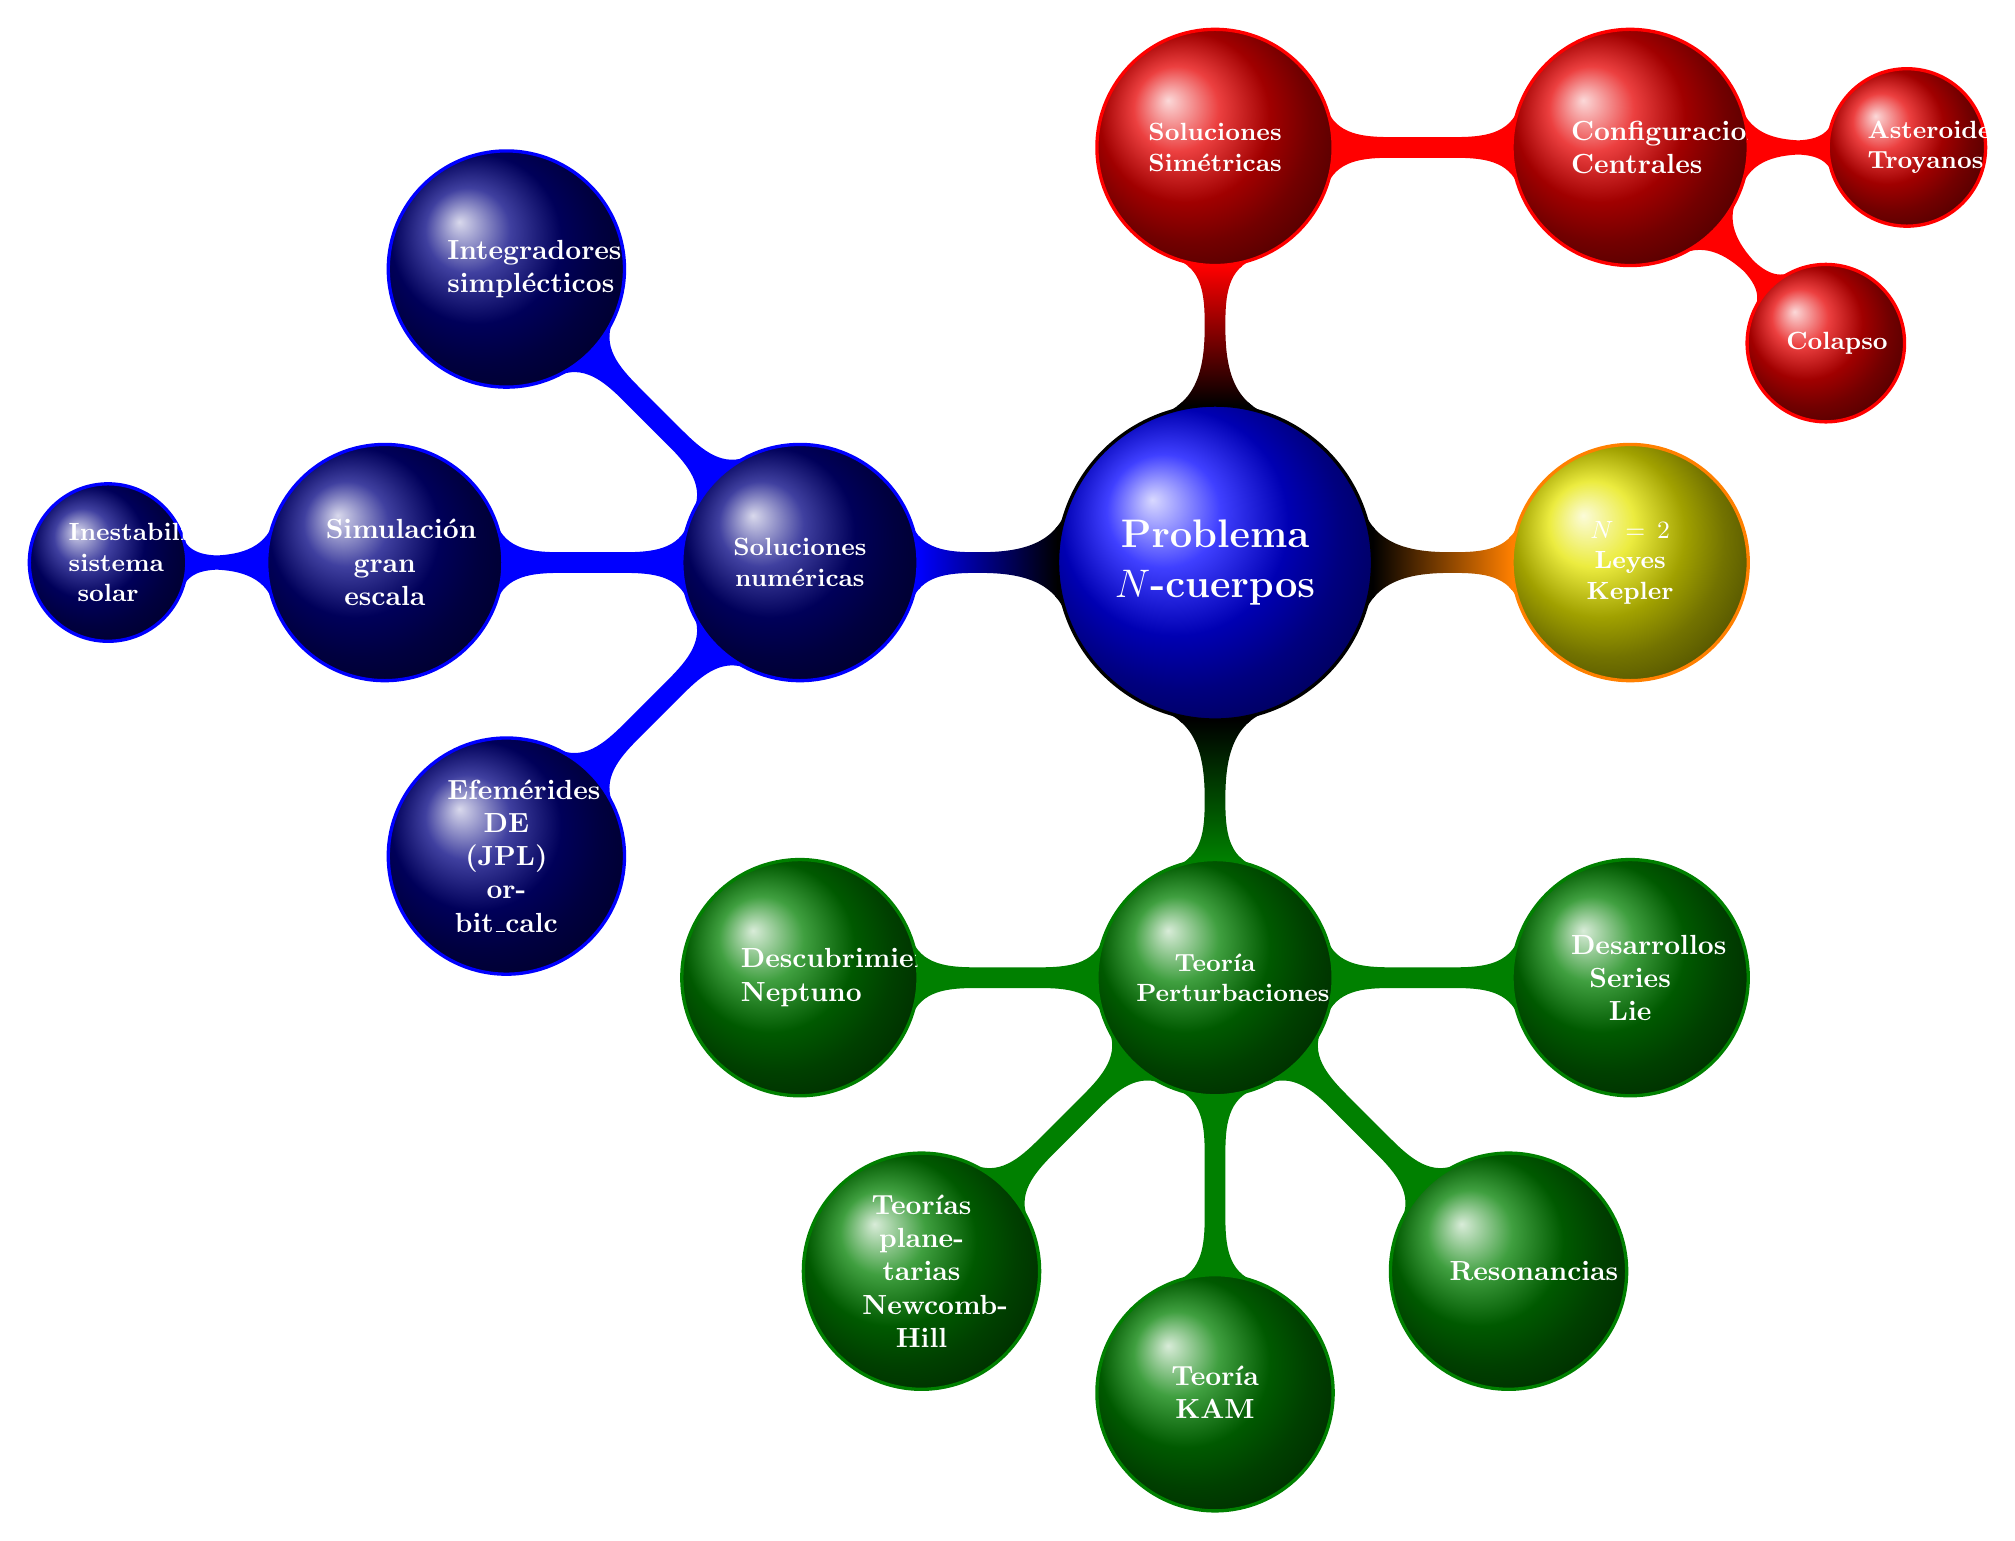
\begin{tikzpicture}
  \path [
    mindmap,
    text = white,
    level 1 concept/.append style =
      {font=\small\bfseries, sibling angle=90,minimum size=3cm,level distance=15em},
    level 2 concept/.append style =
      {font=\normalsize\bfseries,level distance=15em,minimum size=3cm, sibling angle=45},
    level 3 concept/.append style =
      {font=\small\bfseries,level distance=10em,minimum size=2cm,sibling angle=45},
    tex/.style     = {concept, ball color=blue,
      font=\Large\bfseries},
    engines/.style = {concept, ball color=green!50!black},
    formats/.style = {concept, ball color=blue!50!black},
    systems/.style = {concept, ball color=red!90!black},
    editors/.style = {concept, ball color=orange!90!black},%= {concept, ball color=orange!50!black}
    2cuerpos/.style = {concept, ball color=yellow!90!black}
  ]
  node [tex] {Problema\\ $N$-cuerpos} [clockwise from=0]
    child [concept color=orange, nodes={2cuerpos}] {
      node {$N=2$\\Leyes Kepler} }
      child[concept color=green!50!black, nodes={engines}] {
      node {Teoría\\Perturbaciones } [clockwise from=0]
        child { node (A) {Desarrollos Series Lie} }
        child { node {Resonancias} }
        child { node {Teoría KAM} }
        child { node {Teorías planetarias\\Newcomb-Hill} }
       child { node {Descubrimiento\\Neptuno} } }
    child [concept color=blue, nodes={formats}] {
      node {Soluciones numéricas} [counterclockwise from=135]
        child { node {Integradores\\ simplécticos} }
	  child { node {Simulación gran escala}
	  [counterclockwise from=180] child { node {Inestabilidad\\sistema solar}}
	  }
        child { node {Efemérides\\ DE (JPL) orbit\_calc} }}
    child [concept color=red, nodes={systems}] {
      node {Soluciones\\Simétricas} [clockwise from=0]
           child { node {Configuraciones\\Centrales} [counterclockwise from=-45]
          child { node {Colapso} }
          child { node {Asteroides\\Troyanos} }}}
;
\end{tikzpicture}
\end{document}